\documentclass{article}
\usepackage[margin=1in]{geometry}      % default margins are too big
\usepackage{graphicx}                  % for \includegraphics
\usepackage{listings}                  % for typesetting source code
\lstset{language=Python}
\usepackage{mathtools}                 % for better typesetting of math
%\usepackage[round]{natbib}                    % for using different bibliography styles
\bibliographystyle{ieeetr}  
\usepackage{url}
%\usepackage{amsmath}

\usepackage{caption}
\usepackage{subcaption}
\usepackage{listings}
\usepackage{color}

\definecolor{dkgreen}{rgb}{0,0.6,0}
\definecolor{gray}{rgb}{0.5,0.5,0.5}
\definecolor{mauve}{rgb}{0.58,0,0.82}

\lstset{frame=tb,
  language=Java,
  aboveskip=3mm,
  belowskip=3mm,
  showstringspaces=false,
  columns=flexible,
  basicstyle={\small\ttfamily},
  numbers=none,
  numberstyle=\tiny\color{black},
  keywordstyle=\color{black},
  commentstyle=\color{black},
  stringstyle=\color{black},
  breaklines=true,
  breakatwhitespace=true
  tabsize=3
}                 % for typesetting source code

\begin{document}

\title{Implementation Report-3\\
Offloading Decision Process using Reinforcement Learning with Neural Network (RL with NN)}

\author{Aditya Khune}
\date{\today}  % Leave this line out to use the current date.
\maketitle

%%%%%%%%%%%%%%%%%%%%%%%%%%%%%%%%%%%%%%%%%%%%%%%%%%%%%%%%%%%%%%%%%%%%%%

\tableofcontents

%%%%%%%%%%%%%%%%%%%%%%%%%%%%%%%%%%%%%%%%%%%%%%%%%%%%%%%%%%%%%%%%%%%%%%
% Abstract wont come in table of contents! 2

\begin{abstract}
In this implementation I have used Neural Network with Reinforcement Learning to create a decision engine prototype for the offloading process. Reinforcement learning is learning by interacting with an environment. 
\par
I have developed a Neural Network code in Python and have demonstrated results produced by the prototype of Reinforcement Learning offloading app engine.
I have explained how the offloading decision process can benefit from Reinforcement Learning and also presented different scenarios where it can be applicable in \cite{adityaRL}.
\end{abstract}

%%%%%%%%%%%%%%%%%%%%%%%%%%%%%%%%%%%%%%%%%%%%%%%%%%%%%%%%%%%%%%%%%%%%%%


%%%%%%%%%%%%%%%%%%%%%%%%%%%%%%%%%%%%%%%
\section{Mechanism}
Consider an application for which we want to train the $Q$ function for various instances of following parameters:
\begin{itemize}
   \item Bandwidth = Speed Low, Speed Normal, Speed High
   \item WiFi = available, not available
   \item Data transfered = Data Small, Data Medium, Data Big
   \item CPU instance = CPU Low, CPU Normal, CPU High
\end{itemize}

We need to train our $Q$ function in all these conditions. In each such instance our smartphone will have three actions to choose from which are
\begin{itemize}
   \item Local Processing
   \item Offload on Local Servers
   \item Offload on Remote Servers
\end{itemize}
After choosing any of these actions, the smartphone will record the battery units consumed during the processing of the application. The reinforcements will be assigned depending upon the battery consumption. The action which gave us best performance will be the one which consumed least battery units. So we are minimizing our battery units consumption here.\par

A function called $Q$ function stores the reinforcement values for each case it encounters, I have explained about it in my previous report \cite{adityaRL}. In this implementation my main task was to train the $Q$ function using Neural Network. Some more mathematics about this $Q$ function which is used in RL algorithm is shown here:
\subsection{Q Function}
The state-action value function is a function of both state and action and its value is a prediction of the expected sum of future reinforcements. We will call the state-action value function $Q$.
\begin{align*}
      Q(s_t,a_t) \approx \sum_{k=0}^\infty r_{t+k+1}
\end{align*}

here $s_t$ = state, $a_t$ = actions, and $r_t$ = reinforcements received.
This is usually formulated as the least squares objective:


    \begin{align*}
      \text{Minimize } \mathrm{E} \left ( \sum_{k=0}^\infty r_{t+k+1} - Q(s_t,a_t)\right )^2
    \end{align*}
    

%%%%%%%%%%%%%%%%%%%%%%%%%%%%%%%%%%%%%%%%%%%%%%%%%%%%%%%%%%%%%%%%%%%%%%
%\section{Implementation and Results}
%
%\subsection{Scenario 1}
%In this scenario I have considered the parameters that I had used to create a fuzzy logic decision engine in my earlier Implementation report \cite{adityaFL}. Consider an application for which we want to train the $Q$ function for various instances of following parameters:
%\begin{itemize}
%   \item Bandwidth = Speed Low, Speed Normal, Speed High
%   \item WiFi = available, not available
%   \item Data transfered = Data Small, Data Medium, Data Big
%   \item CPU instance = CPU Low, CPU Normal, CPU High
%\end{itemize}
%
%We need to train our $Q$ function in all these conditions. In each such instance our smartphone will have three actions to choose from which are
%\begin{itemize}
%   \item Local Processing
%   \item Offload on Local Servers
%   \item Offload on Remote Servers
%\end{itemize}
%After choosing any of these actions, the smartphone will record the battery units consumed during the processing of the application. The reinforcements will be assigned depending upon the battery consumption. The action which gave us best performance will be the one which consumed least battery units. So we are minimizing our battery units consumption here.\par
%
\section{Implementation}
I have explained the basic idea behind using Reinforcement Learning in the offloading decision process in detail in \cite{adityaRL}.
In this section we will see some code and the plots showing some relevant results.
\subsection{Code}
I have developed a Python code to demonstrate this algorithm. There are three important functions that I am using in this implementation which asre as follows:
\begin{small}
\begin{lstlisting}
def reinforcement(s,sn):
    if sn[0] < 4 and sn[1] == -1:
        r = 0
    elif sn[0] > 3 and sn[0] < 7 and sn[1] == 0:
        r = 0
    elif sn[0] > 6 and sn[1] == 1:
        r = 0
    else:
        r = -1  
    return r       

def initialState():
    initialStates = 0
    process = -1.0
    return np.array([initialStates, process])

def nextState(s,a):
    s = copy.copy(s)
    if s[0] < 10:
        s[0] += 1 #location
        s[1] = a
    return s

validActions = (-1,0,1)
\end{lstlisting}
\end{small}

The `intialState()' function is where we define the starting point of our user, this state of smartphone can contain parameters like bandwidth, data requirement, CPU instance and others. The `reinforcement(s,sn)' function gives reinforcements for the ideal situations in which parameters are suitable for either offloading or local processing.
In the `validActions' we can see three choices which are as follows:
\begin{itemize}
   \item -1 for Local processing
   \item 0 for Offloading on Local Servers
   \item 1 for Offloading on Remote Servers
\end{itemize}      
%\begin{figure}[h!]
%  \centering
%  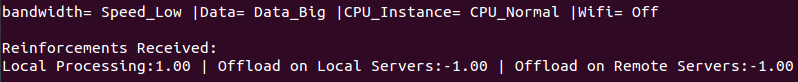
\includegraphics[width=5in]{RL_Local.png}
%  \caption{Best Action: Local Processing}
%  \label{fig:RL_Local}
%\end{figure}
%\begin{figure}[h!]
%  \centering
%  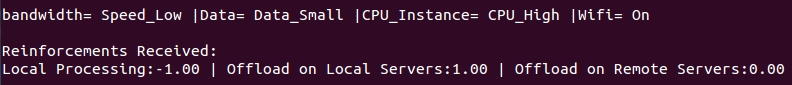
\includegraphics[width=5in]{RL_offload_Local.png}
%  \caption{Best Action: Offload on Local servers, Second best action: Offload on remote Server}
%  \label{fig:RL_offload_Local}
%\end{figure}
%\begin{figure}[h!]
%  \centering
%  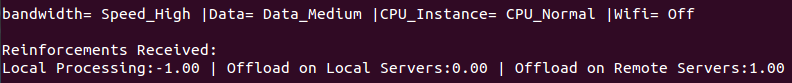
\includegraphics[width=5in]{RL_offload_Remote.png}
%  \caption{Best Action: Offload on Remote servers, Second best action: Offload on Local Server}
%  \label{fig:RL_offload_Remote}
%\end{figure}
%%%%%%%%%%%%%%%%%%%%%%%%%%%%%%%%%%%%%%%%%%%%%%%%%%%%%%%%%%%%%%%%%%%%%
\subsection{Results}

\begin{figure}[h!]
  \centering
  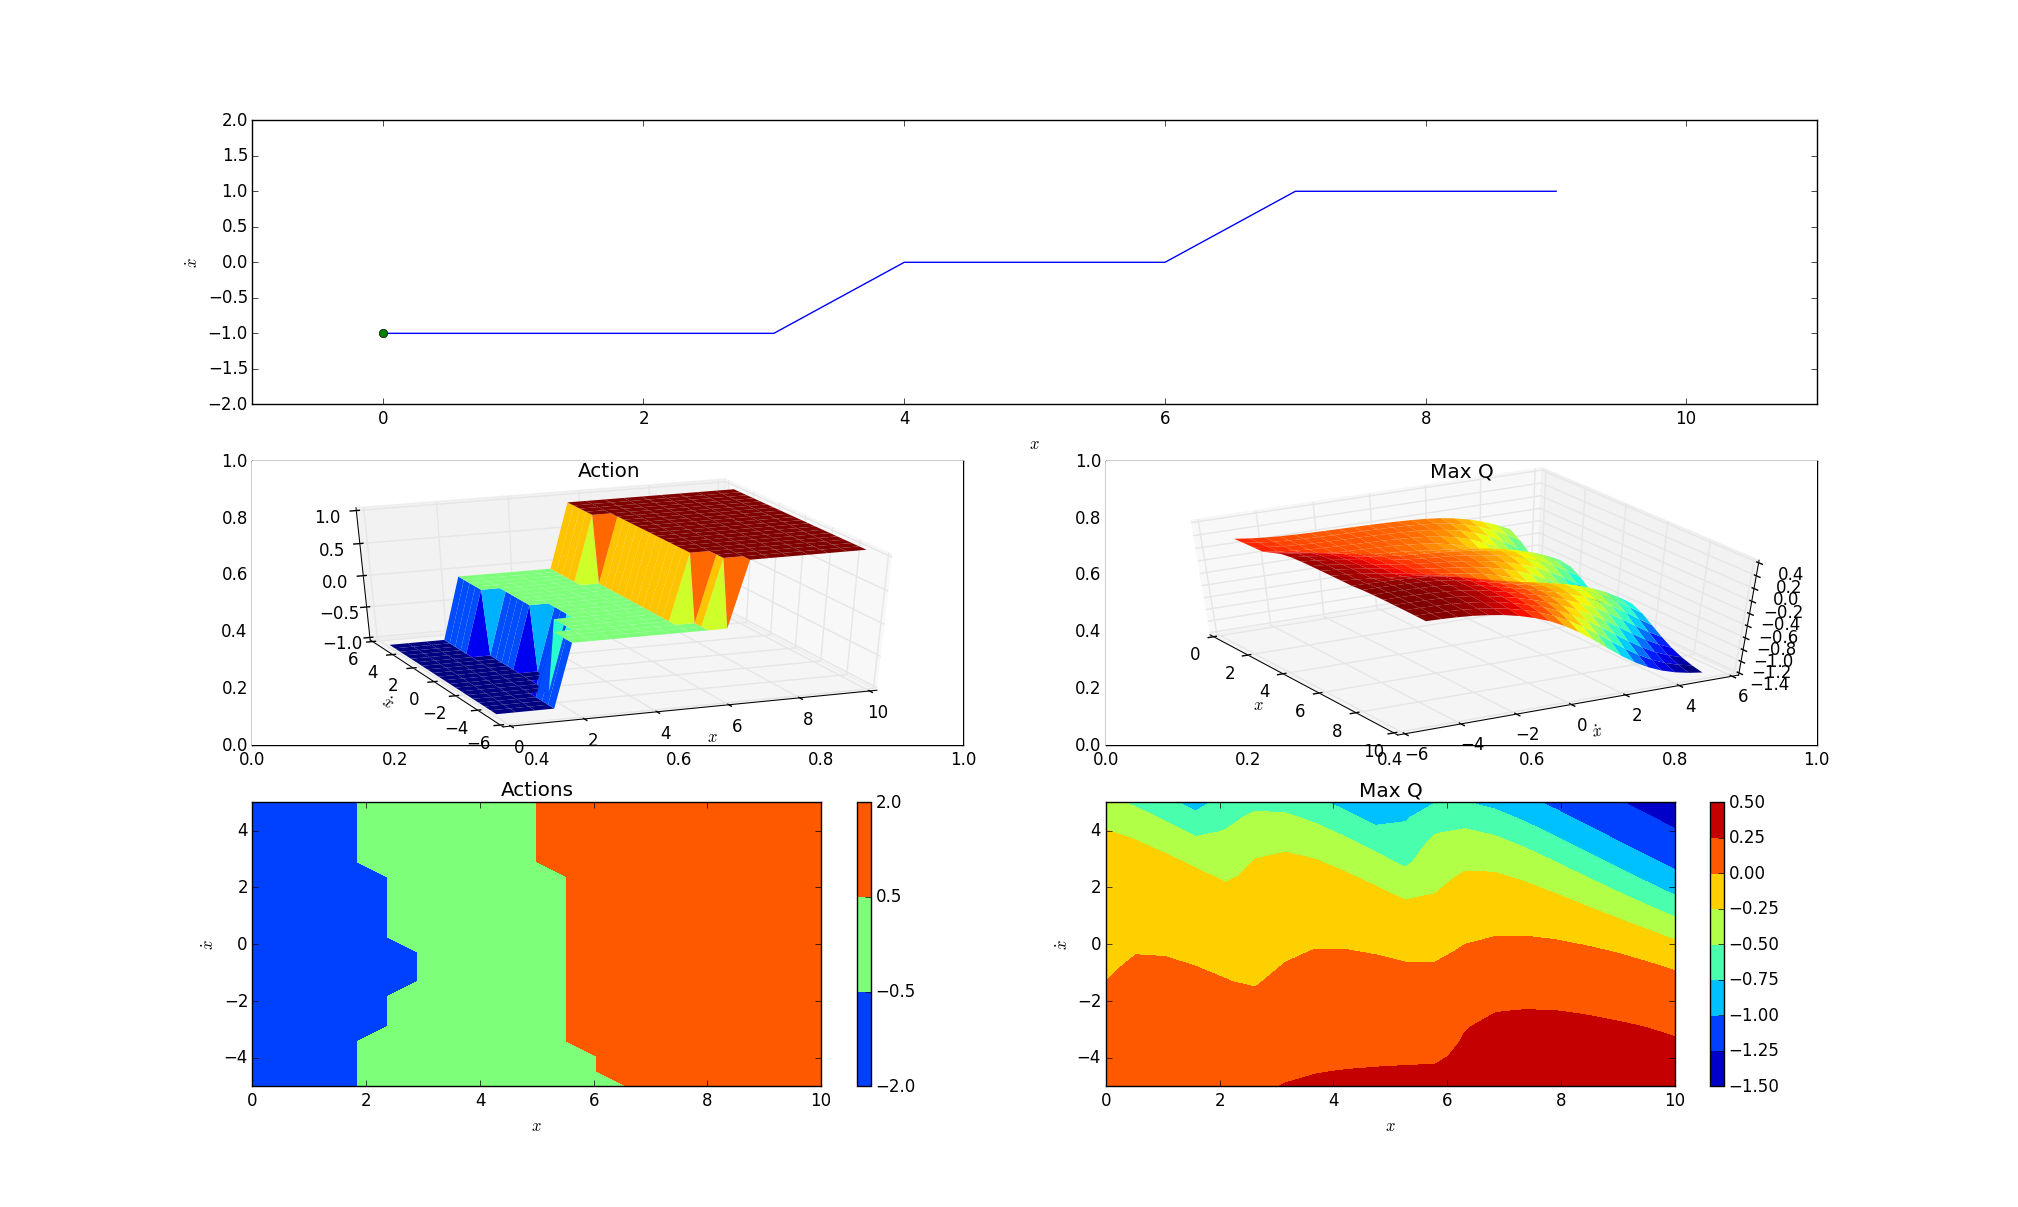
\includegraphics[width=7in]{RL_NN.png}
  \caption{Best Action: Local Processing}
  \label{fig:RL_NN}
\end{figure}
In the figure~\ref{fig:RL_NN} we can see the surface plot of our trained $Q$ function. For these set of results I have customized my Neural Network with no. of hidden layers as (nh) = 5, run for trials (nTrials) = 100 and Steps per trial (nStepsPerTrial) = 10. \par

in the first plot on $x-axis$ we have different locations where the devices is in and location point varies from $0-10$; on $y-axis$ I have plotted the actions recommended by the Q function depending upon the best scenario to save the battery power. So we can see that for location 0, 2 and 3 Local processing is favored by our Q function. When the user moves to different locations between $4-6$ the $Q$ functions choose to Offload the processing on Local servers whereas for locations $6-10$ we should Offload on remote servers. This decision is based on various parameters values present in that location such as `bandwidth available'. \par
In the `Actions' plot we can see 3-D plot with location and Bandwidth parameters. In the `Max $Q$' plot we can see the maximum values that our Q function has for various locations, the Red part is where we got maximum Reinforcement values. 
%%%%%%%%%%%%%%%%%%%%%%%%%%%%%%%%%%%%%%%%%%%%%%%%%%%%%%%%%%%%%%%%%%%%%
%\subsection{Scenario 2}
%In the previous scenario we do not have multiple steps of reinforcements. RL also works in the situation where we have different stages and steps for example in a tic-tac-toe game or even chess. So the previous scenario does not exploit the multiple step option available with RL.\par
%In this second scenario we can envision a situation where we need to further choose from right actions after we have decided whether to offload or not, for example after offloading we might lower the CPU frequency rate of the device to lower the battery consumption, or after offloading we can choose for a specific service that is being offered by the Commercial server provider to get the best of what is available with us and so on.\par
%We can also add time factor as a parameter as sometimes it is seen that the internet speed or performance varies depending which part of day we are using it (because of varying load of users).
%%%%%%%%%%%%%%%%%%%%%%%%%%%%%%%%%%%%%%%%%%%%%%%%%%%%%%%%%%%%%%%%%%%%%%

%\section{Discussion}
%Machine learning algorithms such as Reinforcement Learning with Neural Network and others requires multiple trials for a well trained $Q$ functions which might run into hundreds or thousands of iterations.
%For the compute intensive applications the offloading is beneficial as we have seen in \cite{kumar2010cloud}. For example if we
%want to train a neural network for a smartphone device which has thousands of iterations, we
%can offload he training of Q function on the Cloud, and use the trained function for the decision making.
%
%%%%%%%%%%%%%%%%%%%%%%%%%%%%%%%%%%%%%%%%%%%%%%%%%%%%%%%%%%%%%%%%%%%%%%%
%\section{Next Steps}
%It will be interesting to use Neural Network with Reinforcement Learning, right now I am working on a Python code which will use Neural Network to train the $Q$ function that we studied in this report.\par
%I am also working on an algorithm which uses QDA or LDA Classification techniques for the offloading decision engine. I believe Classification can be useful when applied on the useful data obtained from Reinforcement Learning method, as it requires much lesser calculations than RL, so it will be more efficient.
%%%%%%%%%%%%%%%%%%%%%%%%%%%%%%%%%%%%%%%%%%%%%%%%%%%%%%%%%%%%%%%%%%%%%%%


\bibliographystyle{plainnat}  % or plain, or many other possibilities
\bibliography{bibkrishna3.bib}


\end{document}
